\documentclass{lug}

\title{Computer Graphics \& OpenGL}
\author{Sam Sartor}
\institute{Mines Linux Users Group}

\usepackage{etoolbox}
\usepackage{array}
\usepackage{amsmath}
\usepackage{adjustbox}

\makeatletter
\patchcmd{\beamer@sectionintoc}{\vskip1.5em}{\vskip0.5em}{}{}
\makeatother

\newcommand{\pmidg}[1]{\parbox{\widthof{#1}}{#1}}

\begin{document}

\section{Introduction}

\begin{frame}{Uses}
    \noindent
    \begin{minipage}{.65\textwidth}
        Computer graphics is everywhere!
        \begin{itemize}
            \item Your terminal
            \item Web browsers
            \item Video games
            \item CAD software
            \item Movies, TV Shows
            \item Virtual reality
            \item Your bootloader
            \item QT, GTK+, wxWidgets
            \item Vim, Emacs, Notepad
            \item Embedded devices
        \end{itemize}
    \end{minipage}%
    \begin{minipage}{.35\textwidth}
        \pmidg{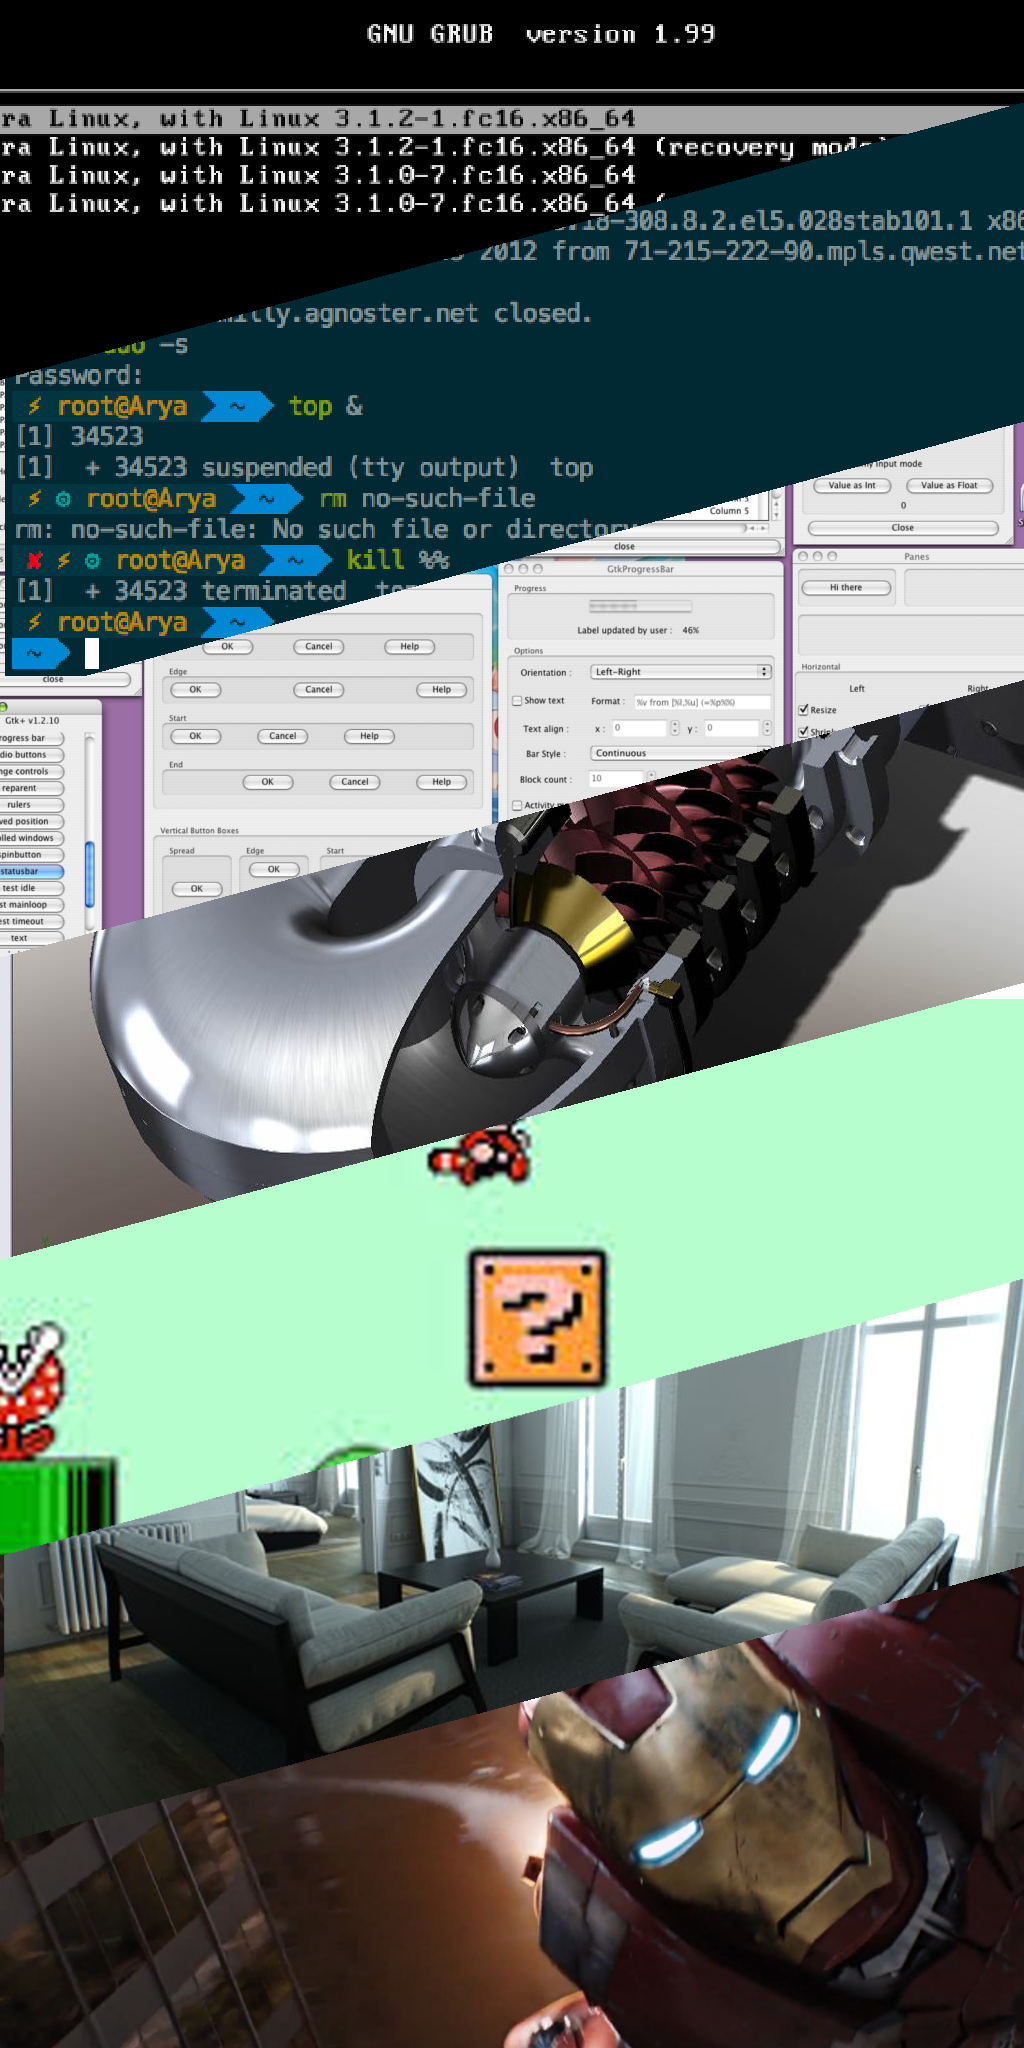
\includegraphics[width=\textwidth]{graphics/uses}}
    \end{minipage}
\end{frame}

\begin{frame}{Definition}
\begin{center}
    \pmidg{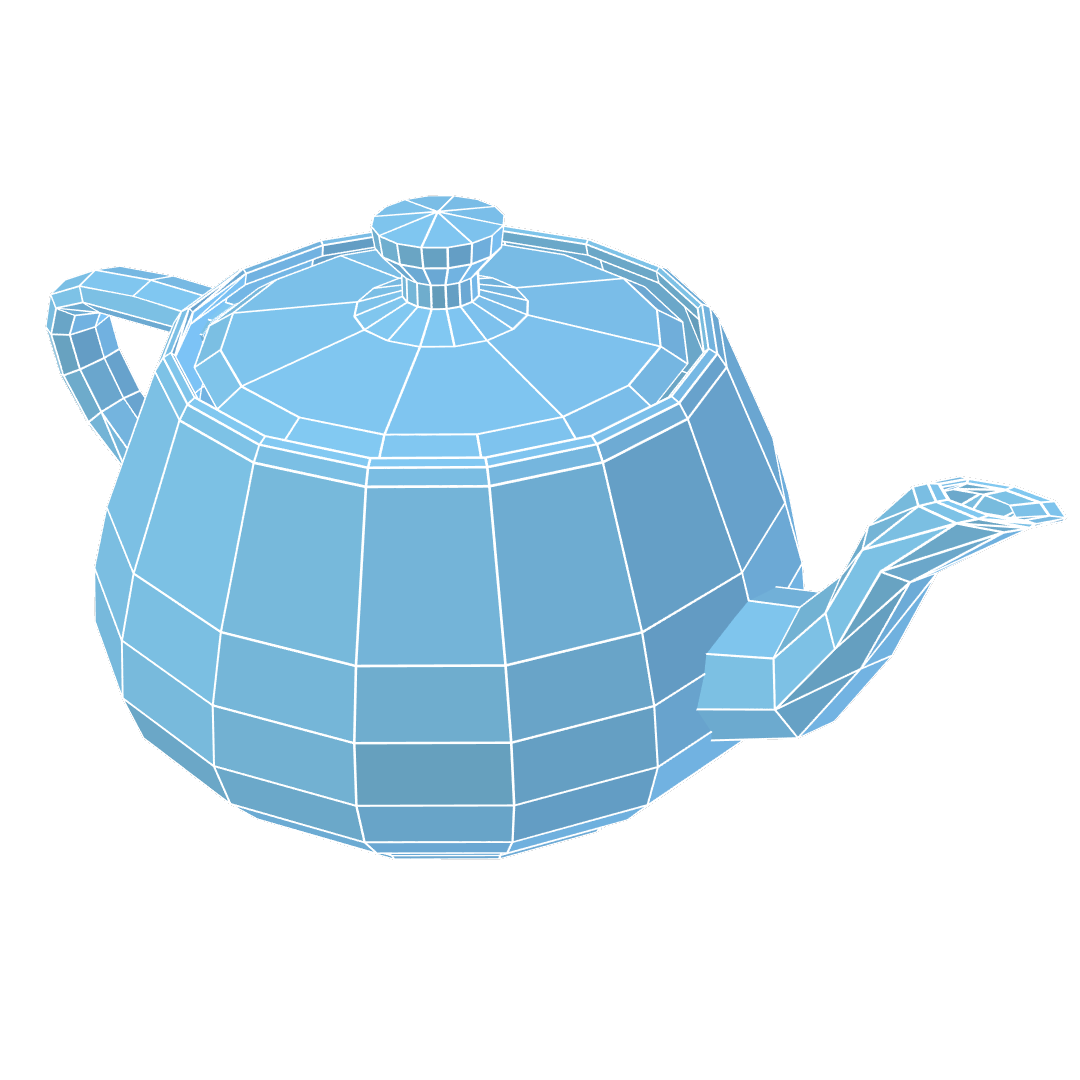
\includegraphics[width=4cm]{graphics/teapot_mesh}} \scalebox{2}{$\rightarrow$} \pmidg{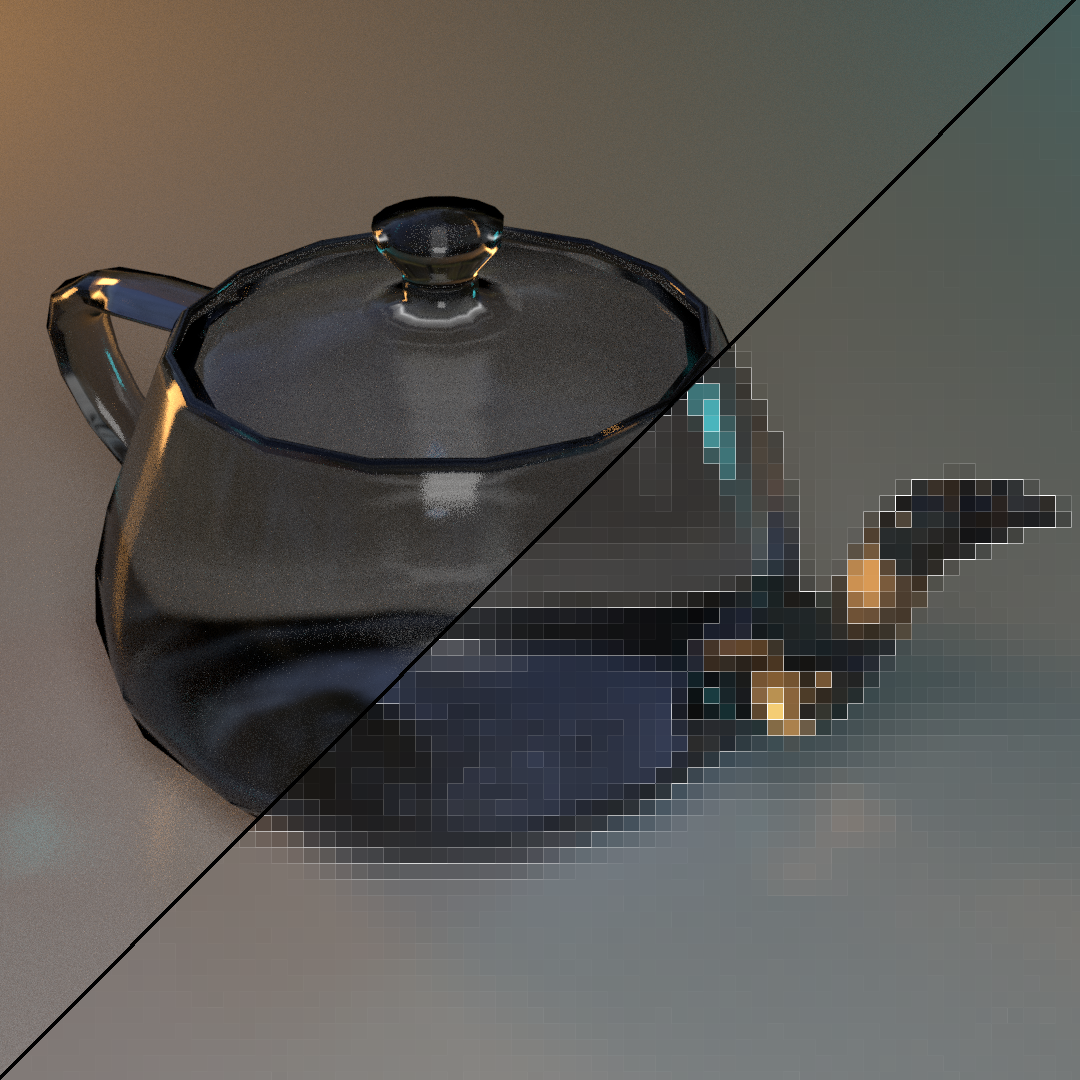
\includegraphics[width=4cm]{graphics/teapot_rt_pix}} \\
    
    \bigskip

    Computer graphics is the science of turning \textit{shapes} into \textit{pixels}. \footnote{Kindof, it can get more interesting than that}
\end{center}
\end{frame}

\section{History}

\begin{frame}{1950s \& 1960s}
    \noindent
    \begin{minipage}{.65\textwidth - 2em}
        \small
        \begin{itemize}
            \item Military used computer controlled oscilloscopes to display strategic information
            \item Very simple graphical CAD programs and visualizers created
            \item Very first computer games
            \item Research into elementary 3D wireframe graphics
            \item Very early raster displays
        \end{itemize}
    \end{minipage}%
    \hspace{1.5em}%
    \begin{minipage}{.35\textwidth}
        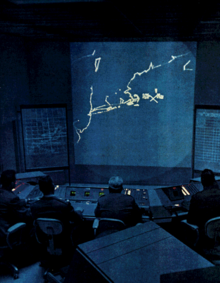
\includegraphics[width=\textwidth]{graphics/sage_control} \\
        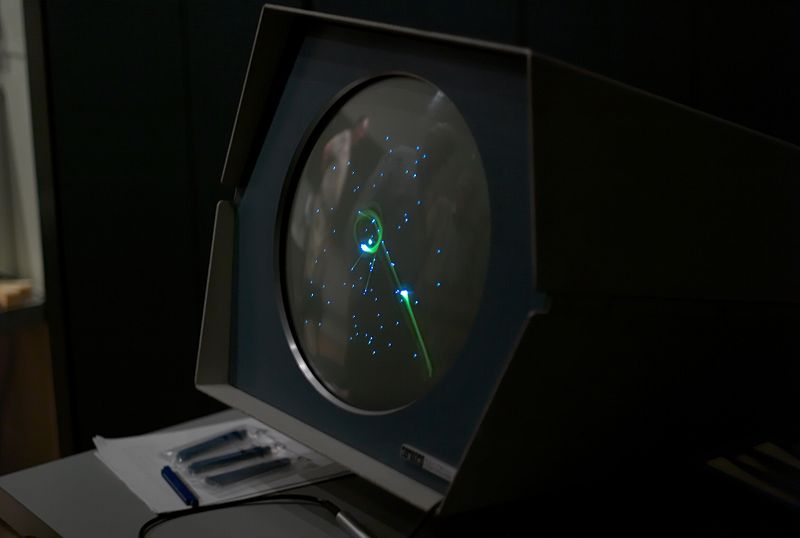
\includegraphics[width=\textwidth]{graphics/spacewar}
    \end{minipage}
\end{frame}

\begin{frame}{1970s \& 1980s}
    \noindent
    \begin{minipage}{.65\textwidth - 2em}
        \small
        \begin{itemize}
            \item Basic lighting models such as Phong developed
            \item Low-res, 2D games become commercially available
            \item CGI starts to be used in Movies such as 1982's \textit{Wrath of Khan} and 1985's \textit{Young Sherlock Holmes}
            \item Modern GUIs are developed
            \item High-quality digital typesetting becomes commonplace
        \end{itemize}
    \end{minipage}%
    \hspace{1.5em}%
    \begin{minipage}{.35\textwidth}
        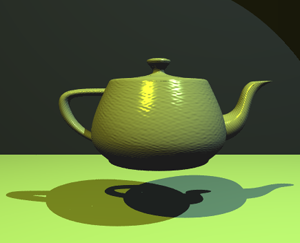
\includegraphics[width=\textwidth]{graphics/teapot_70s} \\
        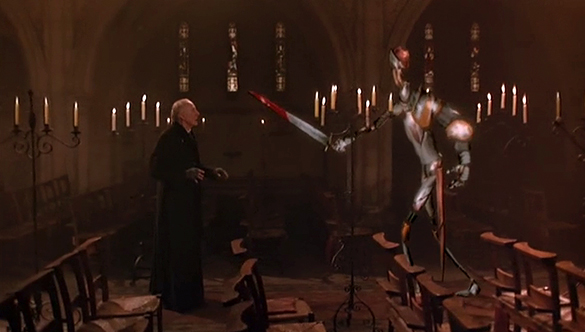
\includegraphics[width=\textwidth]{graphics/ysh_knight} \\
        
\includegraphics[width=\textwidth]{graphics/postscript_text}
    \end{minipage}
\end{frame}

\begin{frame}{1990s \& 2000s}
    \noindent
    \begin{minipage}{.65\textwidth - 2em}
        \small
        \begin{itemize}
            \item Fidelity and performance are immensely increased
            \item Personal computers, 3D video games, and GUIs become ubiquitous
            \item OpenGL and Direct3D standardize hardware graphics support
            \item CGI becomes commonplace in Movies, advertisements, and TV 
            \item Global illumination and physically based rendering (PBR) techniques developed
        \end{itemize}
    \end{minipage}%
    \hspace{1.5em}%
    \begin{minipage}{.35\textwidth}
        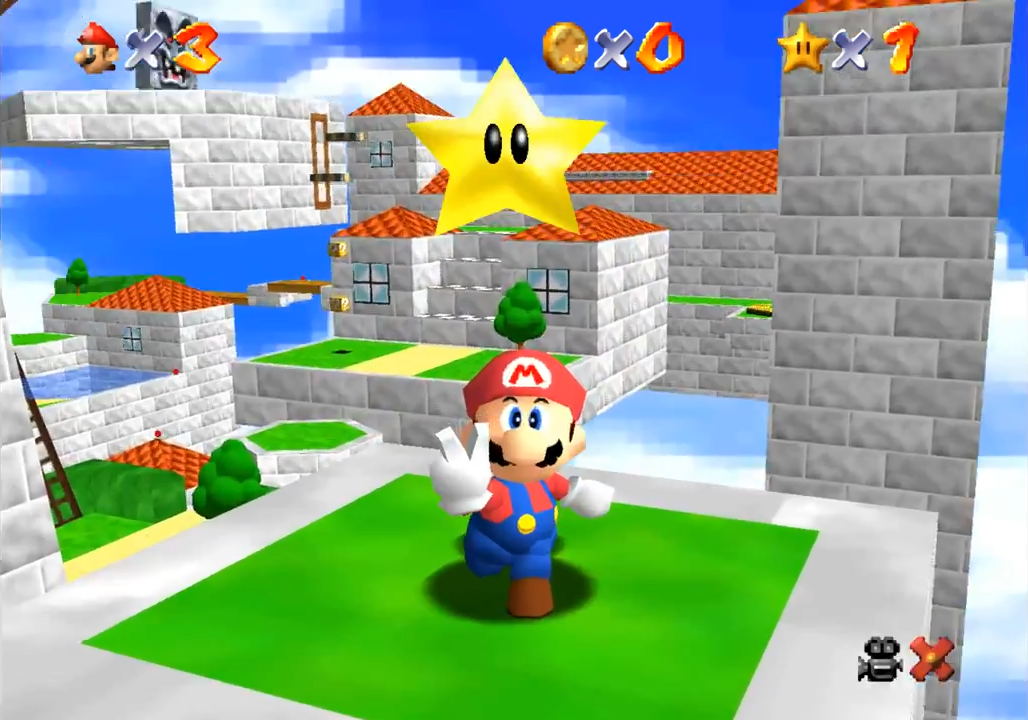
\includegraphics[width=\textwidth]{graphics/supermario64} \\
        
\includegraphics[width=\textwidth]{graphics/toy_story} \\
        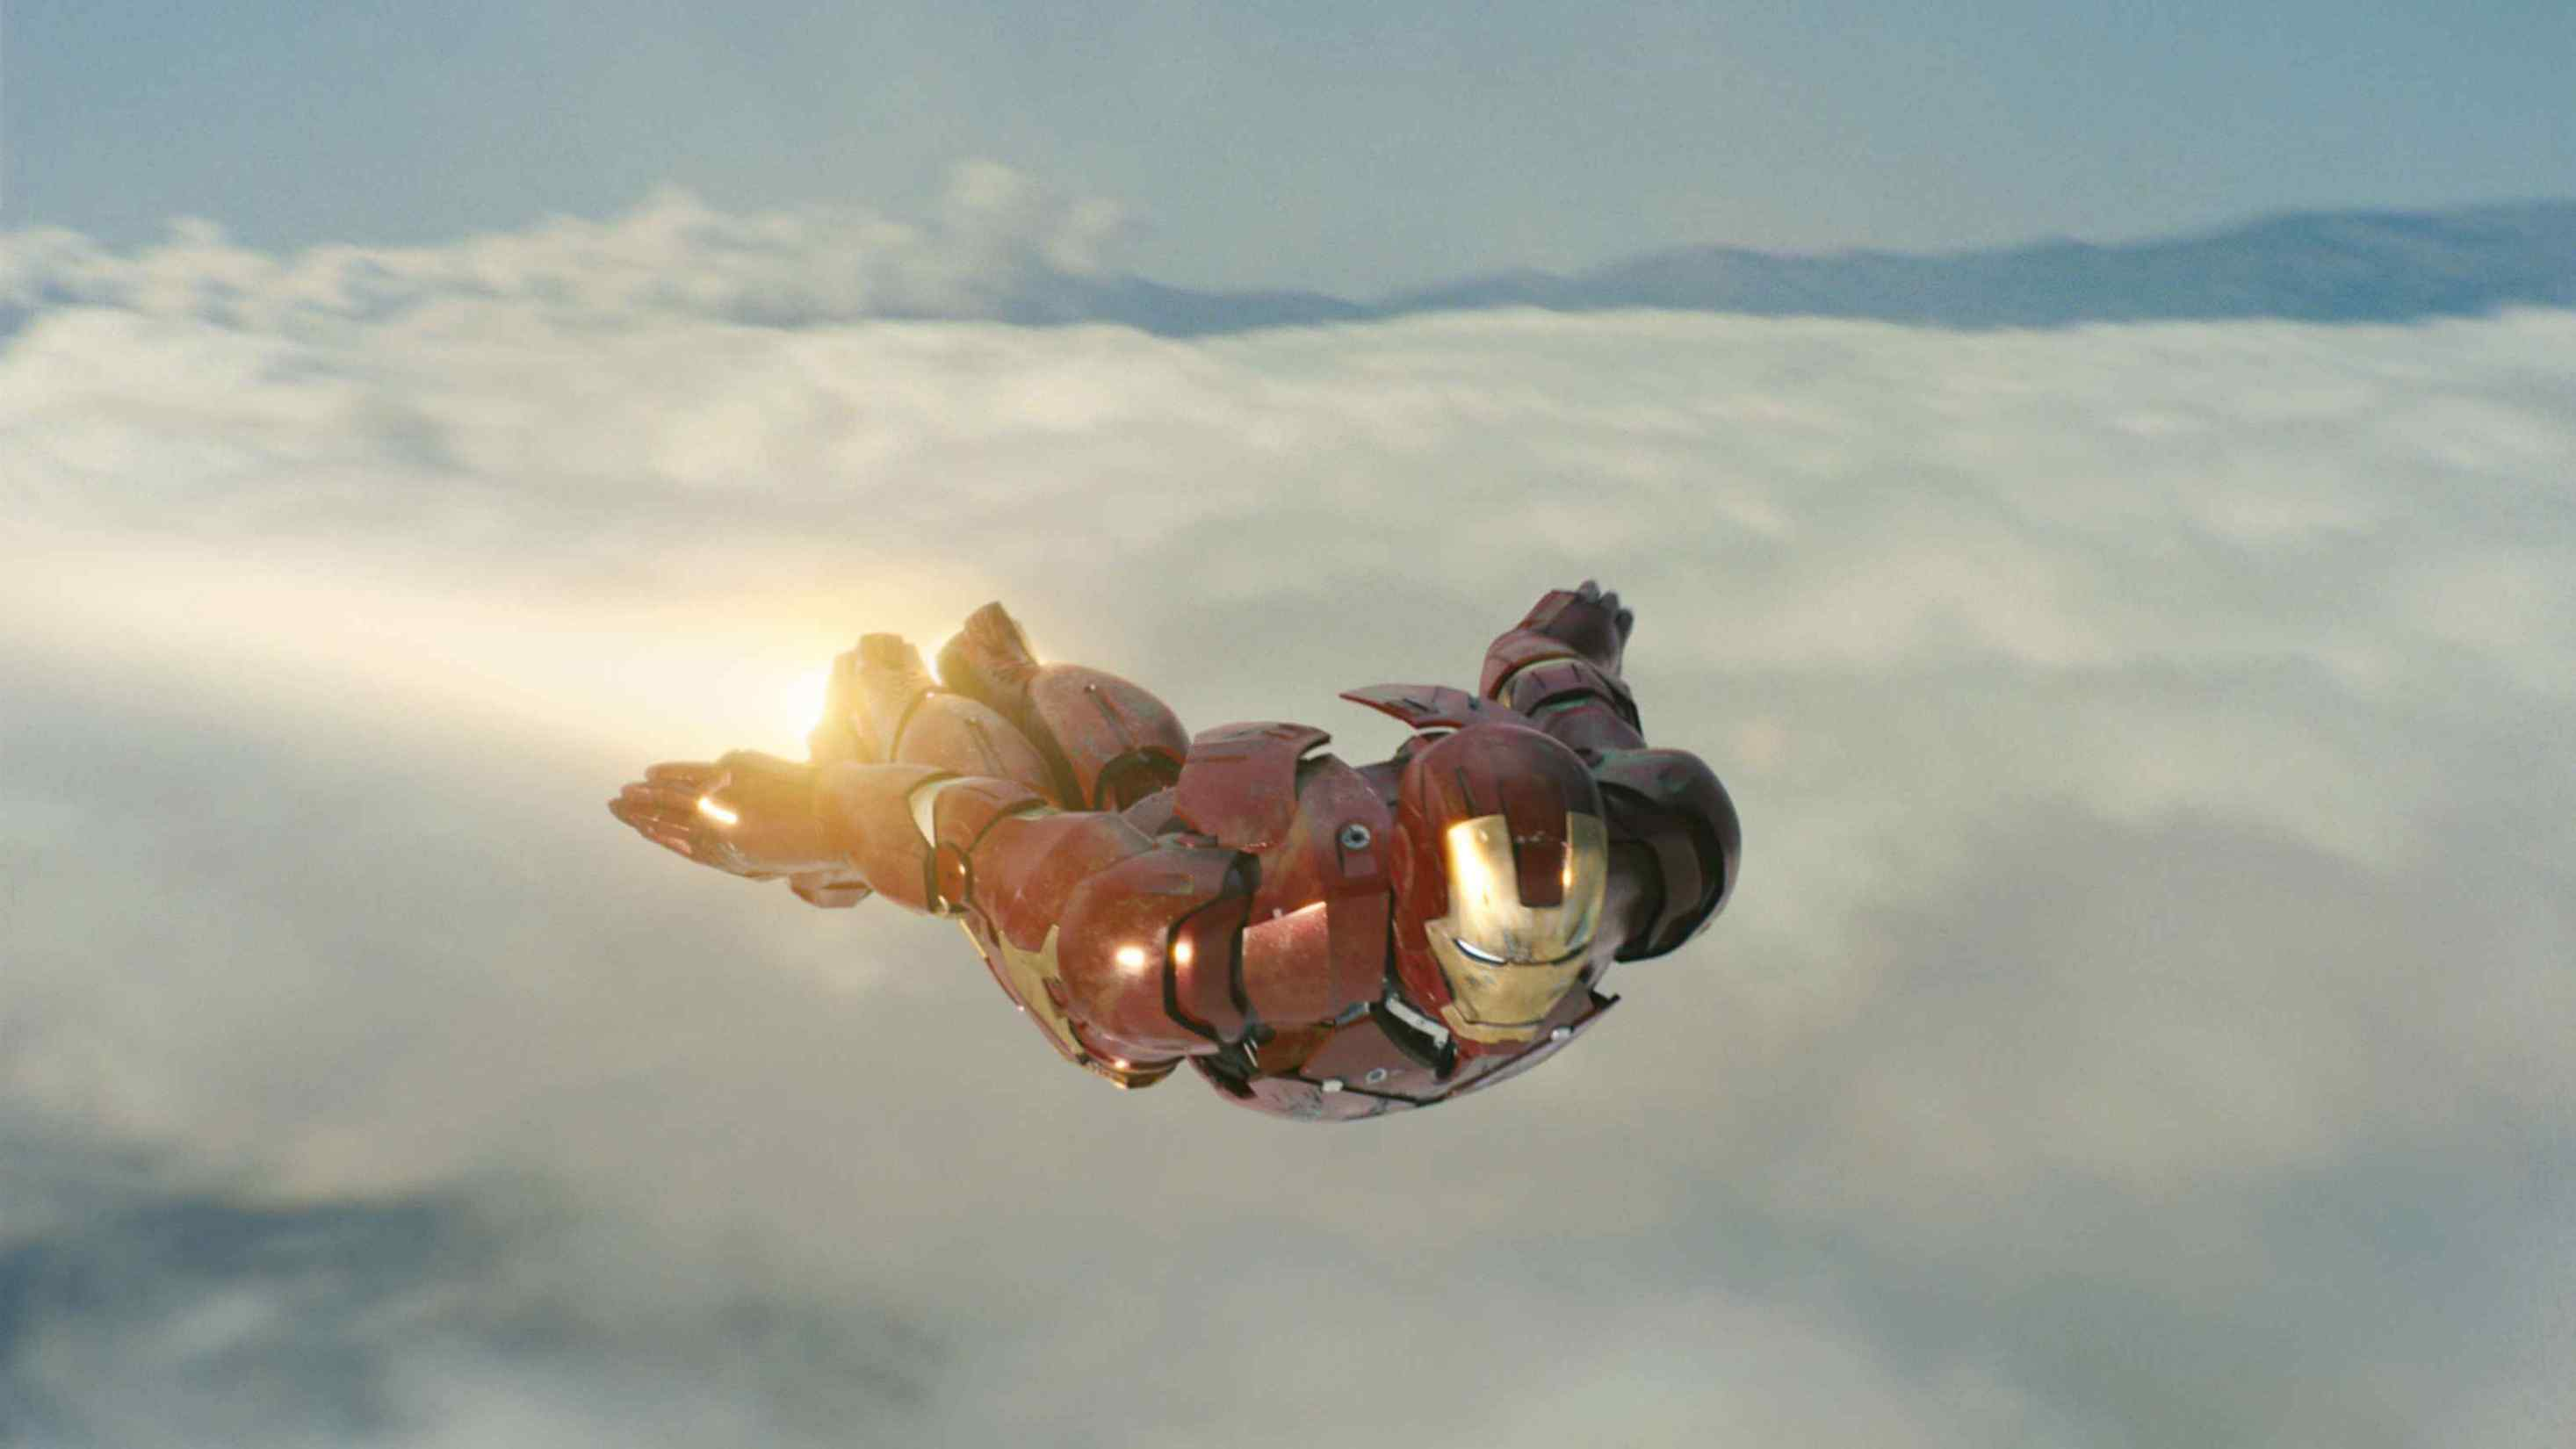
\includegraphics[width=\textwidth]{graphics/iron_man_2008}
    \end{minipage}
\end{frame}

\begin{frame}{Today}
    \noindent
    \begin{minipage}{.65\textwidth - 2em}
        \small
        \begin{itemize}
            \item Given enough time, budget and expertise, offline graphics are photorealistic
            \item Particle and fluid simulations are extremely fast and accurate
            \item Realtime graphics make extensive use of shaders and PBR techniques
            \item UIs and offline graphics are increasingly GPU accelerated
            \item Linux and Mac have improved support for games and graphical software
        \end{itemize}
    \end{minipage}%
    \hspace{1.5em}%
    \begin{minipage}{.35\textwidth}
        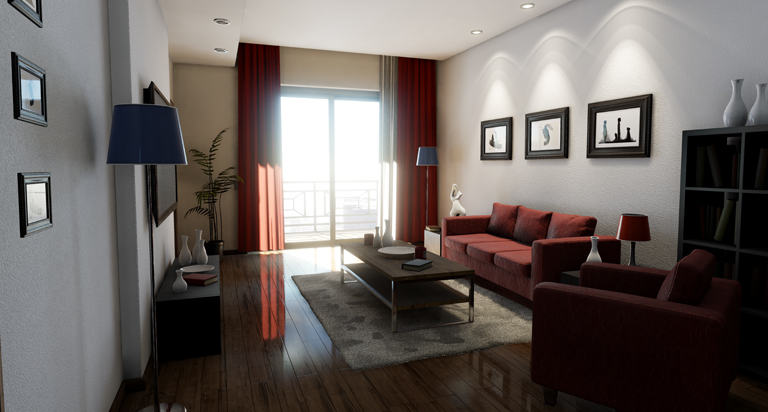
\includegraphics[width=\textwidth]{graphics/unreal4_damn} \\
        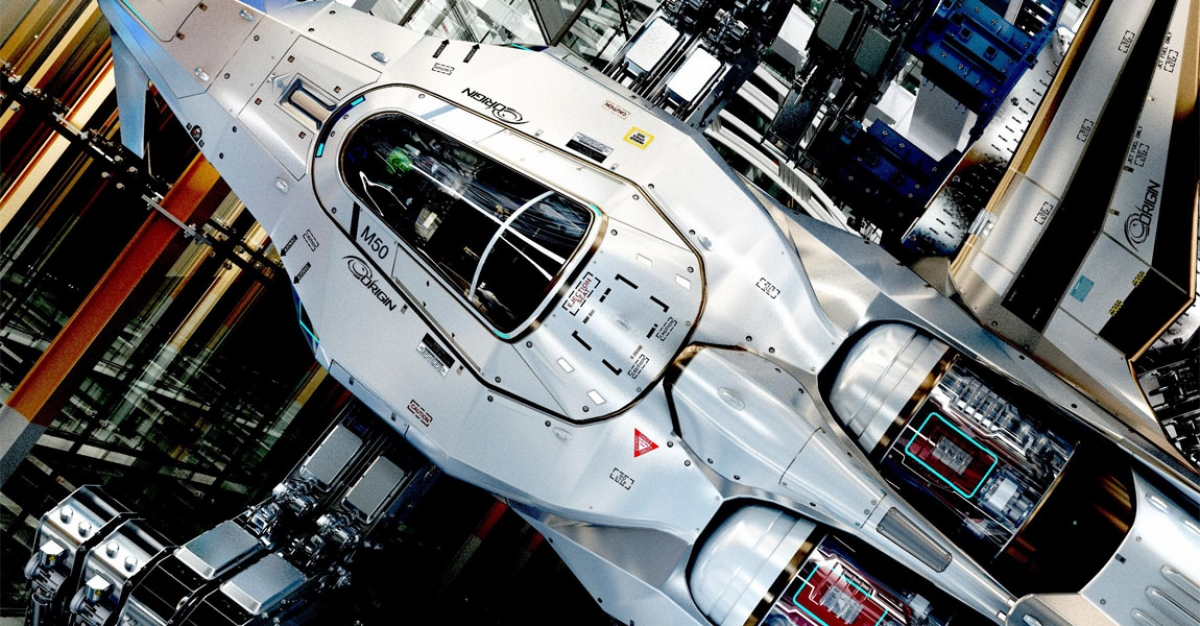
\includegraphics[width=\textwidth]{graphics/star_citizen_pbr} \\
        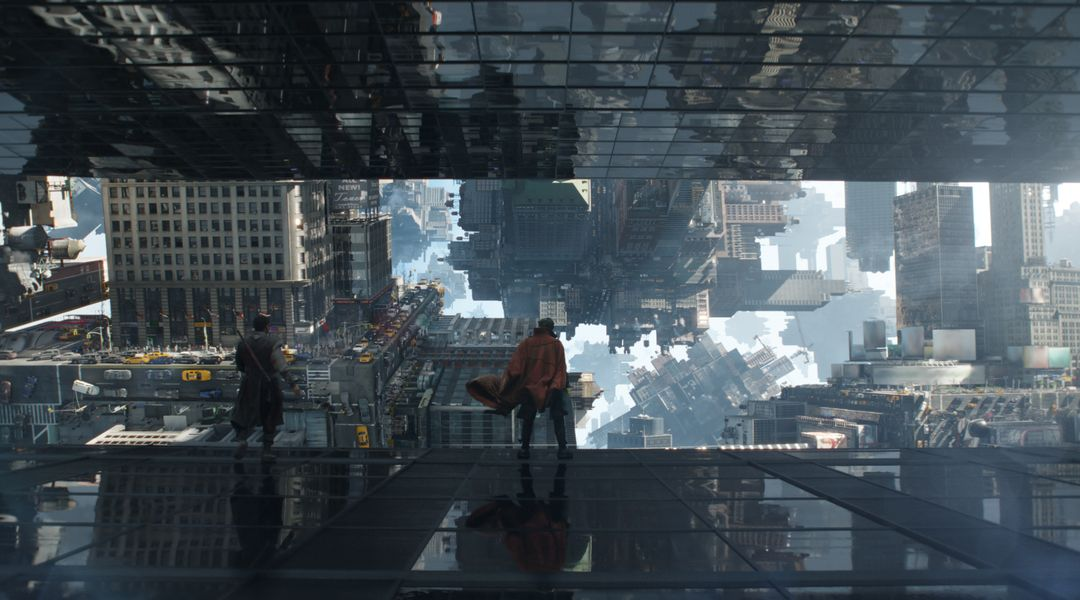
\includegraphics[width=\textwidth]{graphics/dr_strange} \\
        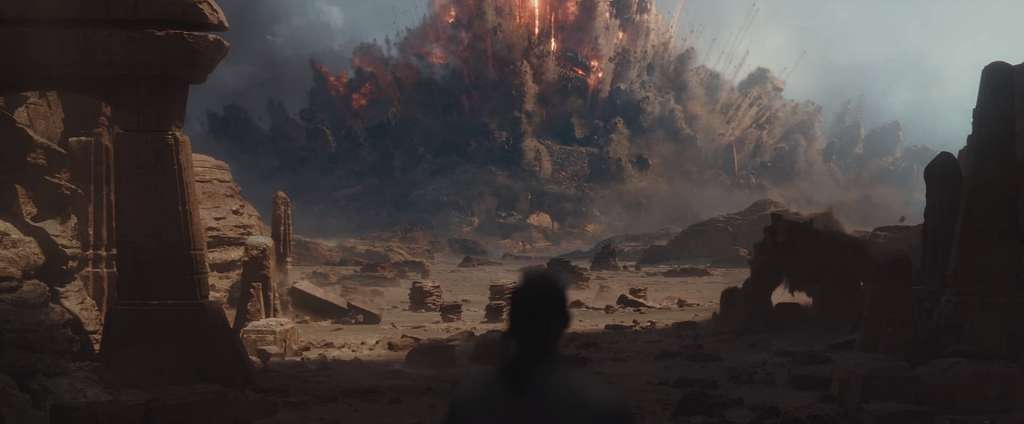
\includegraphics[width=\textwidth]{graphics/rogue_one_boom}
    \end{minipage}
\end{frame}

\section{Behind the Scenes}

\begin{frame}{Realtime}
    \noindent
    \begin{minipage}{.7\textwidth - 1.5em}
        \small

        Realtime graphics use OpenGL or Direct3D to rasterize and shade
        triangular geometry on a graphics card/chip. Performance is very
        important due to the high framerate that is required for smooth
        gameplay/interactivity/animation. Lighting and materials focus on
        being "good enough" rather than on being truly accurate.

    \end{minipage}%
    \hspace{1.5em}%
    \begin{minipage}{.3\textwidth}
        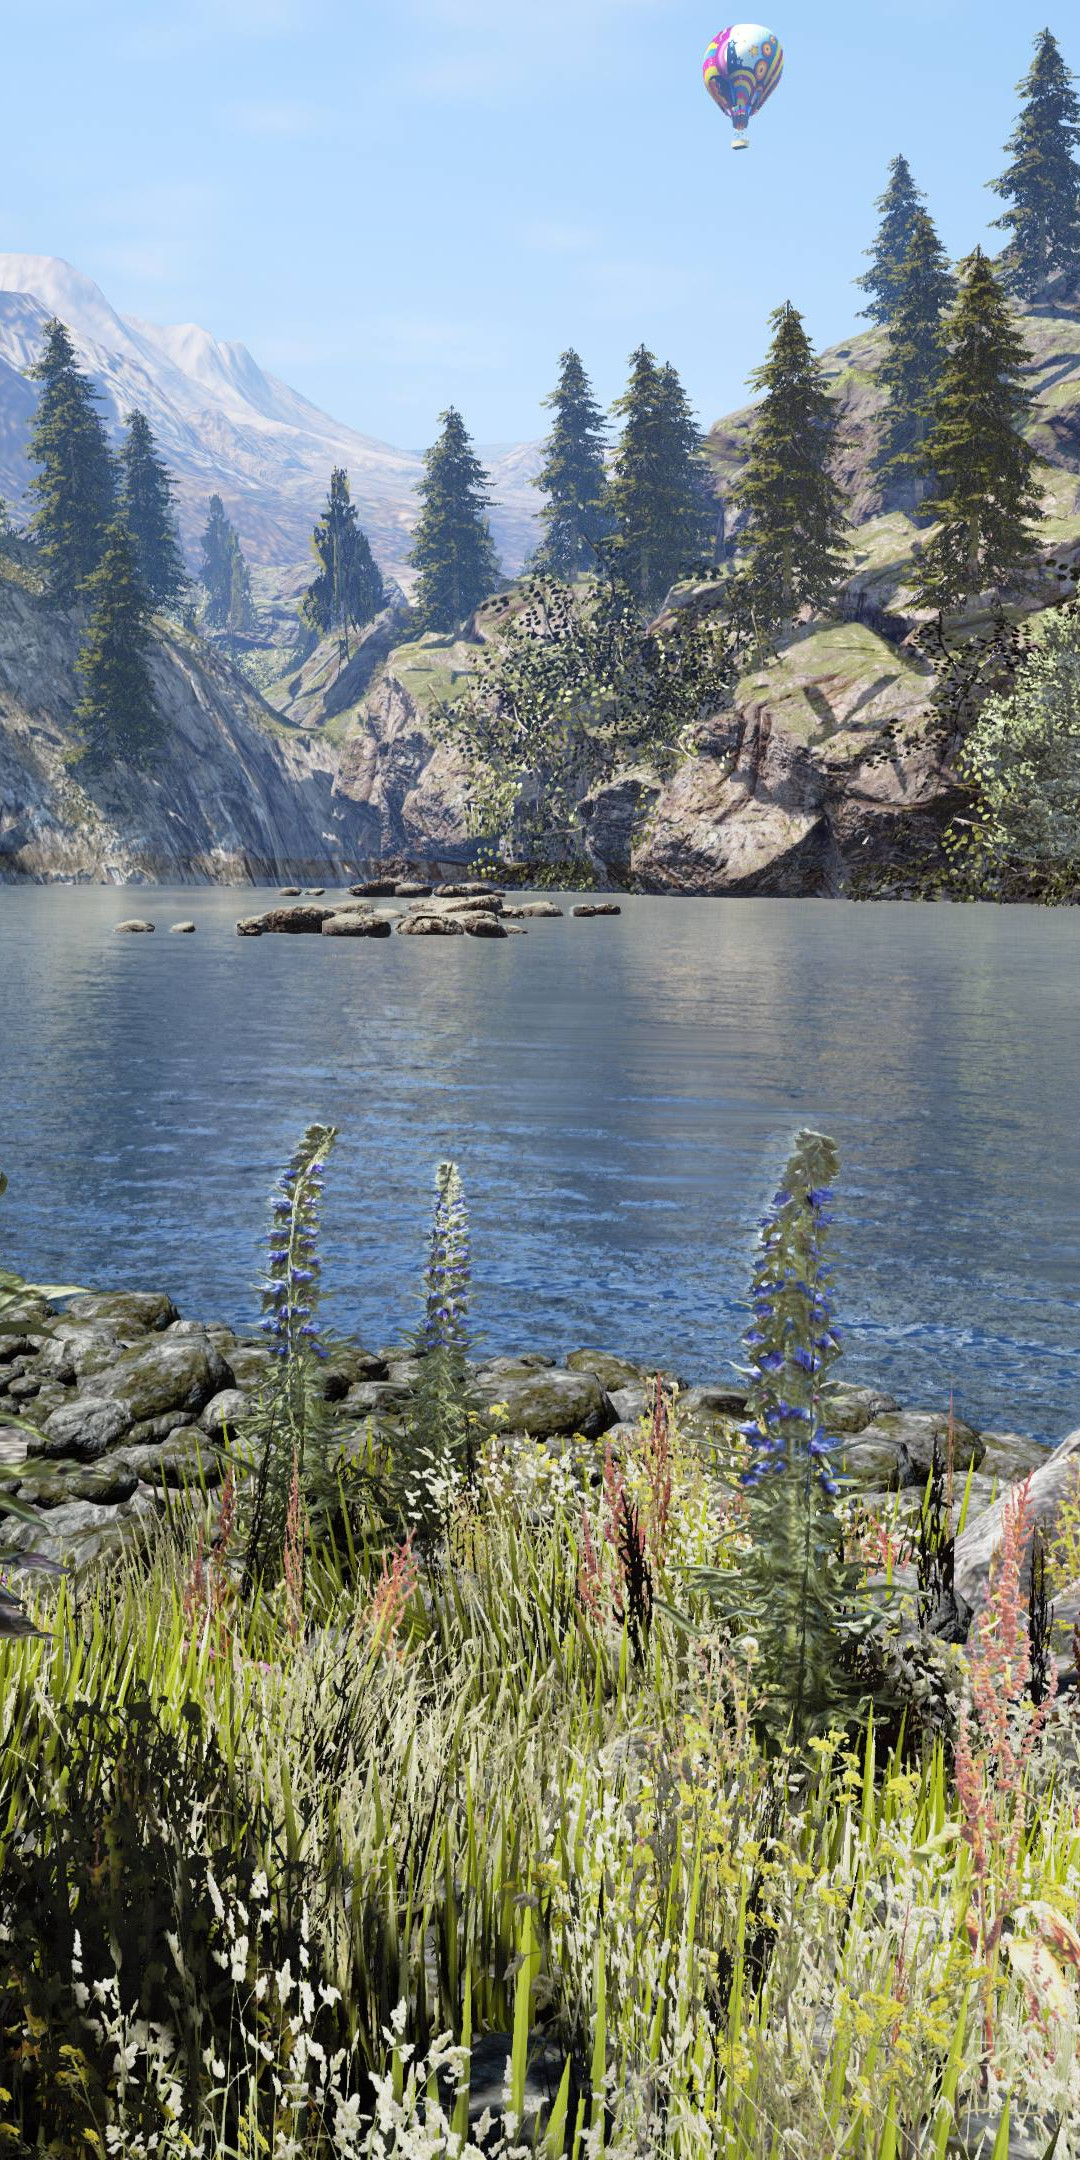
\includegraphics[width=\textwidth]{graphics/game_graphics}
    \end{minipage}
\end{frame}

\begin{frame}{UIs}
    \noindent
    \begin{minipage}{.7\textwidth - 1.5em}
        \small

        While they look different, UIs generally use OpenGL or Direct3D as
        well. Everything is still made of textured \& shaded triangles. Anti-%
        aliasing, text fidelity, etc. are all more important while lighting
        effects are generally absent. Responsiveness is key, but the frame can
        be updated as needed, not every 30th of a second.

    \end{minipage}%
    \hspace{1.5em}%
    \begin{minipage}{.3\textwidth}
        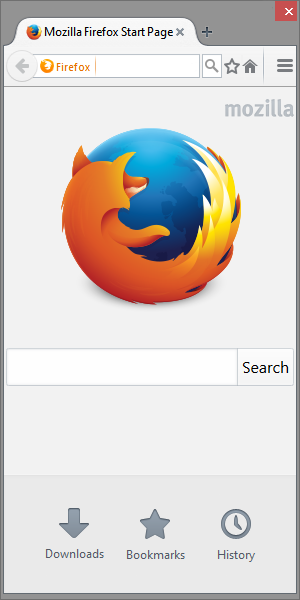
\includegraphics[width=\textwidth]{graphics/firefox_start}
    \end{minipage}
\end{frame}

\begin{frame}{Offline}
    \noindent
    \begin{minipage}{.7\textwidth - 1.5em}
        \small

        Offline graphics are used when the medium is non-interactive (movies,
        advertisements, etc). Because the available resources are limited only
        by budget and patience, offline graphics have unmatched fidelity. CPUs
        are often used instead of GPUs because this allows for more advanced
        calculations. However, this comes at a cost. Individual frames may
        take days to render.

    \end{minipage}%
    \hspace{1.5em}%
    \begin{minipage}{.3\textwidth}
        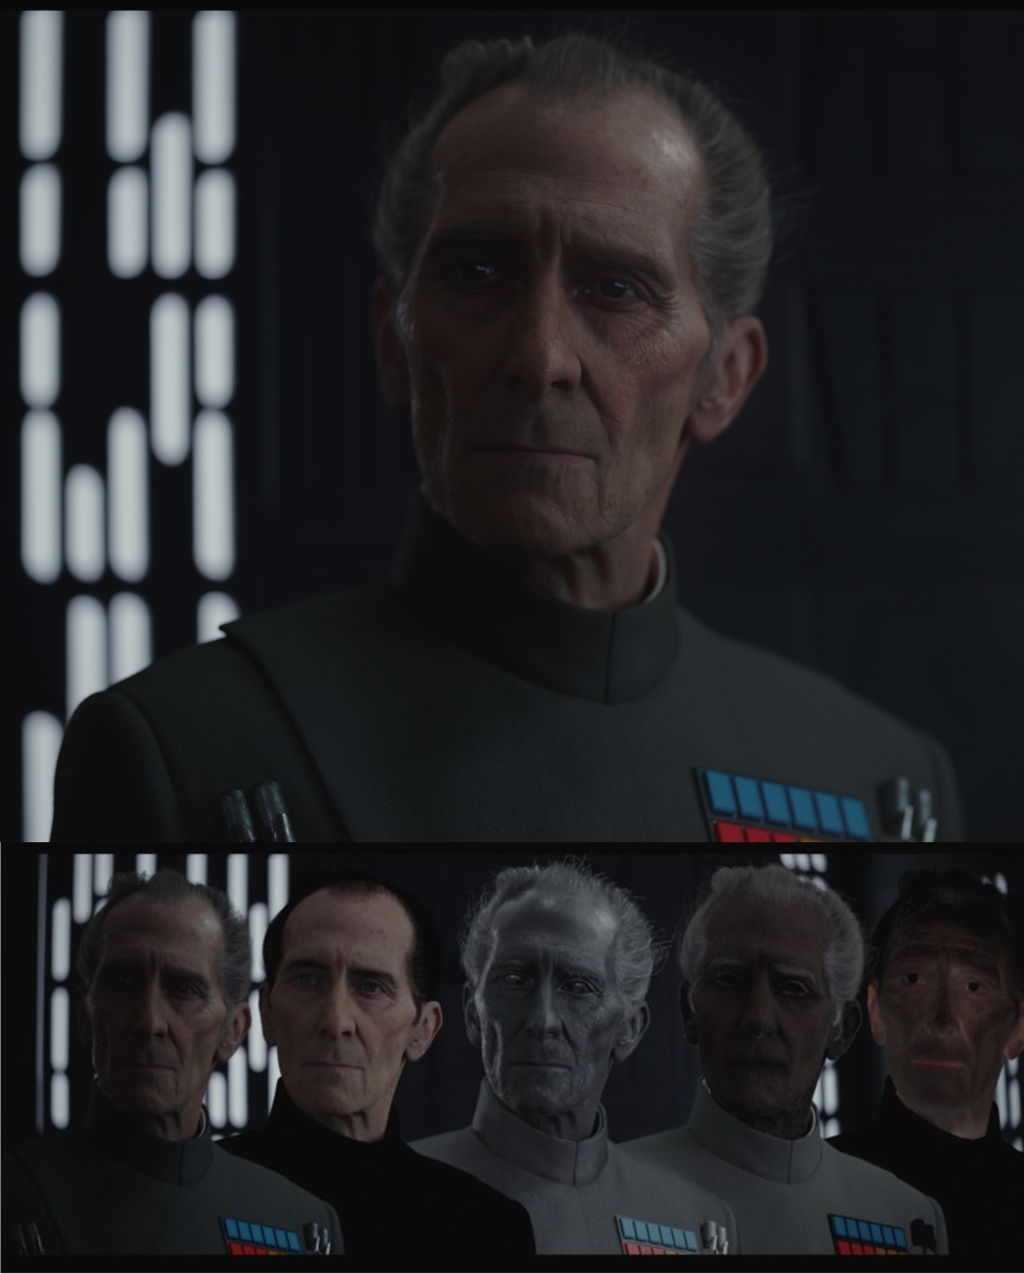
\includegraphics[width=\textwidth]{graphics/tarkin_combo} \\
        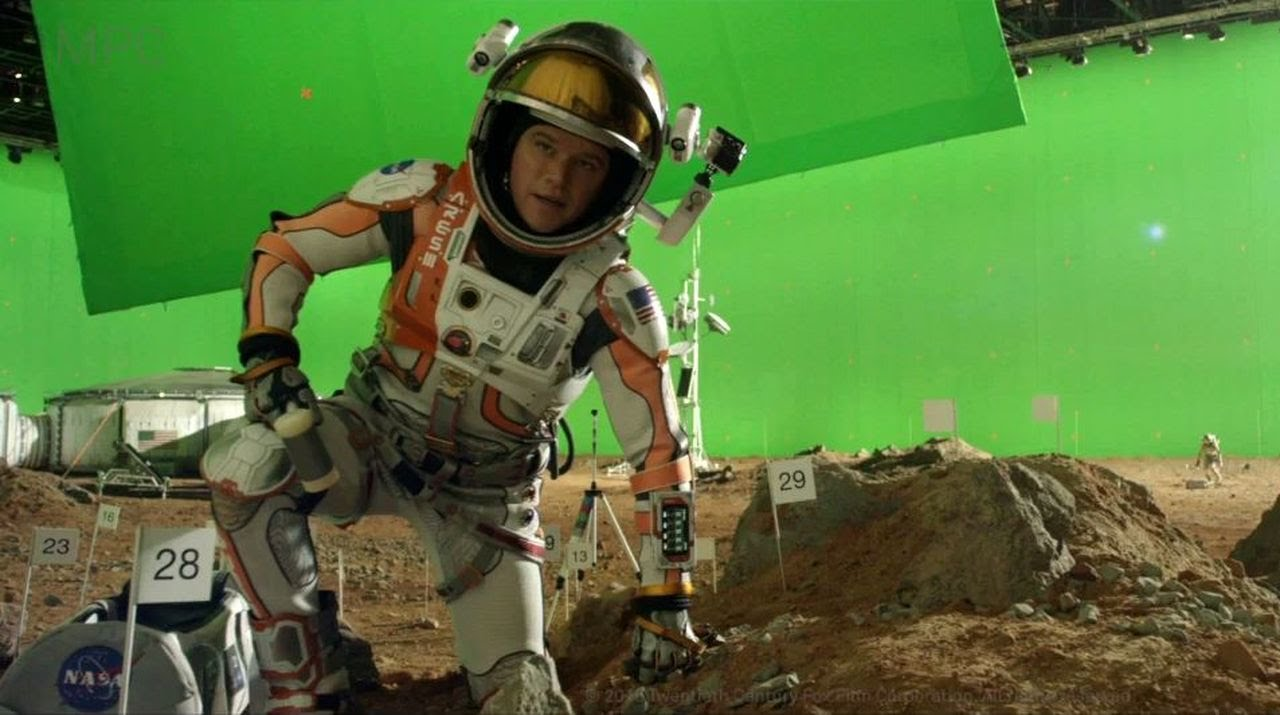
\includegraphics[width=\textwidth]{graphics/green_mars}
    \end{minipage}
\end{frame}